\documentclass[]{article}

% Imported Packages
%------------------------------------------------------------------------------
\usepackage{amssymb}
\usepackage{amstext}
\usepackage{amsthm}
\usepackage{amsmath}
\usepackage{enumerate}
\usepackage{fancyhdr}
\usepackage[margin=1in]{geometry}
\usepackage{graphicx}
\usepackage{extarrows}
%\usepackage{setspace}
%------------------------------------------------------------------------------

% Header and Footer
%------------------------------------------------------------------------------
\pagestyle{plain}  
\renewcommand\headrulewidth{0.4pt}                                      
\renewcommand\footrulewidth{0.4pt}                                    
%------------------------------------------------------------------------------

% Title Details
%------------------------------------------------------------------------------
\title{Deliverable \#2 Template}
\author{SE 3A04: Software Design II -- Large System Design}
\date{}                               
%------------------------------------------------------------------------------

% Document
%------------------------------------------------------------------------------
\begin{document}

\maketitle	

\section{Introduction}
\label{sec:introduction}
% Begin Section

This section should provide an brief overview of the entire document.

\subsection{Purpose}
\label{sub:purpose}
% Begin SubSection
\begin{enumerate}[a)]
	\item Delineate the purpose of the document
	\item Specify the intended audience for the document
\end{enumerate}
% End SubSection

\subsection{System Description}
\label{sub:system_description}
% Begin SubSection
\begin{enumerate}[a)]
	\item Give a brief description of the system. This could be a paragraph or two to give some context to this document.
\end{enumerate}
% End SubSection

\subsection{Overview}
\label{sub:overview}
% Begin SubSection
\begin{enumerate}[a)]
	\item Describe what the rest of the document contains 
	\item Explain how the document is organised
\end{enumerate}
% End SubSection

% End Section

\section{Use Case Diagram}
%\label{sec:use_case_diagram}
\begin{figure}
	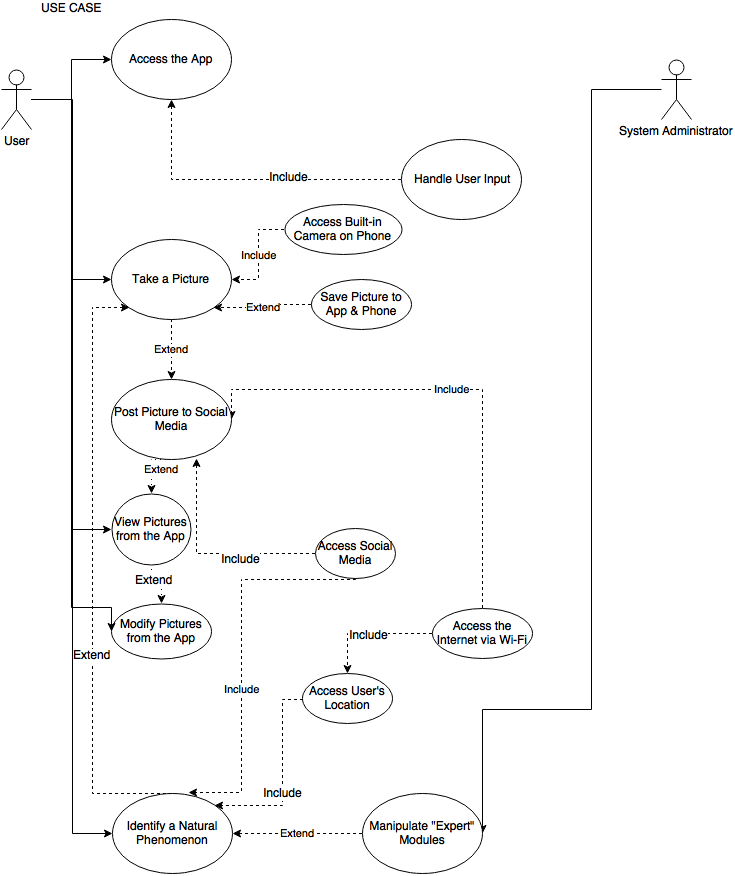
\includegraphics[width=\linewidth]{usecase.pdf}
	\caption{Use Case Diagram}
\end{figure}
\begin{enumerate}
	\item User wishes to access the app.  The user shall be able to download the app onto their smart phone in order to access it.  This downloading action will be handled by the operating system.  User shall be able to open the app.  The system developer needs to ensure that application shall be able to handle user input, so that the user can access and interact with the app.
	\item User wishes to take a picture and post it to social media.  User can then access the built-in camera on phone and it's functionality from the app.  User can also save the picture to the app and the phone if they so desire.  User shall be able to post to social media directly from the app.  The system developer shall ensure that application can access the internet via wireless connection from smart phone, the built-in camera on the smart phone, and social media (Instagram).  Application shall be able to save pictures directly to the phone.
	\item User wishes to view and modify pictures from the app.  User shall be able to view saved pictures through the app and the phone.  User shall be able delete pictures from the app and the phone.  System Developer shall ensure that application can display requested pictures to the user.  Application shall be able to delete pictures directly on the phone.
	\item User wishes to identify a natural phenomena. User shall be able to post a picture on social media through the app.  The system developer shall ensure that the app can access the user's location using google maps services. App shall have access to the internet via wireless connection from smart phone. App shall be able to switch "expert" modules in order to identify the natural phenomenon. 
\end{enumerate}
% End Section

\section{Analysis Class Diagram}
\label{sec:analysis_class_diagram}
% Begin Section
This section should provide an analysis class diagram for your application.
% End Section


\section{Architectural Design}
\label{sec:architectural_design}
% Begin Section
This section should provide an overview of the overall architectural design of your application. You overall architecture should show the division of the system into subsystems with high cohesion and low coupling.

\subsection{System Architecture}
\label{sub:system_architecture}
% Begin SubSection
\begin{enumerate}[a)]
	\item Identify and explain the overall architecture of your system
	\item Be sure to clearly state the name of the architecture
	\item Provide the reasoning and justification of the choice
	\item Provide a structural architecture diagram showing the relationship among the subsystems (if appropriate)
\end{enumerate}
% End SubSection

\subsection{Subsystems}
\label{sub:subsystems}
% Begin SubSection
NatureOptix will be broken down into six subsystems. These subsystems are
\begin{enumerate}
	\item Controller %x2
	\item Experts x4,
	\item Database.
\end{enumerate}
The first Controller is the subsystem to control\begin{comment}ata between the user and the experts \end{comment} where the data goes. The controller will ask the user a series of questions. It will then take this information and pass it to the four experts. After the experts have returned with the potential answers to determine what phenomenon the user might be seeing, the controller will then present the options to the user. 

The four Experts will be implemented as algorithms. 
\begin{comment}
The second Controller will 
\end{comment}
% End SubSection

% End Section
	
\section{Class Responsibility Collaboration (CRC) Cards}
\label{sec:class_responsibility_collaboration_crc_cards}
% Begin Section
This section should contain all of your CRC cards.

\begin{enumerate}[a)]
	\item Provide a CRC Card for each identified class
	\item Please use the format outlined in tutorial, i.e., 
	\begin{table}[ht]
		\centering
		\begin{tabular}{|p{5cm}|p{5cm}|}
		\hline 
		 \multicolumn{2}{|l|}{\textbf{Class Name:}} \\
		\hline
		\textbf{Responsibility:} & \textbf{Collaborators:} \\
		\hline
		\vspace{1in} & \\
		\hline
		\end{tabular}
	\end{table}
	
\end{enumerate}
% End Section

\appendix
\section{Division of Labour}
\label{sec:division_of_labour}
% Begin Section
Include a Division of Labour sheet which indicates the contributions of each team member. This sheet must be signed by all team members.
% End Section

\newpage
\section*{IMPORTANT NOTES}
\begin{itemize}
%	\item You do \underline{NOT} need to provide a text explanation of each diagram; the diagram should speak for itself
	\item Please document any non-standard notations that you may have used
	\begin{itemize}
		\item \emph{Rule of Thumb}: if you feel there is any doubt surrounding the meaning of your notations, document them
	\end{itemize}
	\item Some diagrams may be difficult to fit into one page
	\begin{itemize}
		\item It is OK if the text is small but please ensure that it is readable when printed
		\item If you need to break a diagram onto multiple pages, please adopt a system of doing so and thoroughly explain how it can be reconnected from one page to the next; if you are unsure about this, please ask about it
	\end{itemize}
	\item Please submit the latest version of Deliverable 1 with Deliverable 2
	\begin{itemize}
		\item It does not have to be a freshly printed version; the latest marked version is OK
	\end{itemize}
	\item If you do \underline{NOT} have a Division of Labour sheet, your deliverable will \underline{NOT} be marked
\end{itemize}


\end{document}
%------------------------------------------------------------------------------